\documentclass[titlepage]{article}
\usepackage{amsmath, amsfonts}
\usepackage{mathtools}
\usepackage[capitalise]{cleveref}
\usepackage[labelfont=bf]{caption}
\usepackage{subcaption}
\usepackage{geometry}
\usepackage{pdflscape}
\usepackage{graphicx}
\usepackage{float}
\usepackage{afterpage}
\usepackage[outdir=../results/plots/]{epstopdf}
\usepackage[section]{placeins}
\usepackage[backend=biber,citestyle=numeric,style=ieee]{biblatex}
\usepackage{siunitx}
\usepackage{booktabs}

\DeclareSourcemap{
  \maps[datatype=bibtex]{
    \map[overwrite=true]{
       \pertype{online}
       \step[fieldset=urldate,fieldvalue={\the\year-\the\month-\the\day}]
    } 
 }
}
\addbibresource{bibliography.bib}

\graphicspath{{../results/plots}}

\sisetup{output-exponent-marker=\ensuremath{\mathrm{e}}}
\DeclareSIUnit{\mph}{mph}

\title{Robust Statistics: Exam Assignment}
\author{Othman El Hammouchi}

\begin{document}

\maketitle

\section*{Question 1}

The sensitivity curves corresponding to the M-estimators of location for Huber's $\rho$ with $b = 1.5$ and Tukey's bisquare with $c = 4.68$ are shown (in red) in \cref{fig:q1-sens-curves-1e2,fig:q1-sens-curves-1e6}. Also plotted (in black) are their influence functions. For a general M-estimator, these are given by
\begin{equation}
  \mathrm{IF}(x, T, F) \coloneqq \frac{\psi(x)}{\int \psi'(y) \, dF(y)} \,,
\end{equation}
as explained on p.\ 12 of Part 2 of the course slides. In the case of Huber's $\rho$, the denominator is given by
\begin{equation}
  \int \psi'(y) \, dF(y) = \int_{-b}^b \, dF(y) = F(b) - F(-b) \,,
\end{equation}
which for $F = \Phi$ is $\approx 0.866$. Similarly, we have
\begin{equation}
  \int \psi'(y) \, dF(y) = \frac{1}{\sqrt{2 \pi}} \int_{-c}^c \left(\left(1 - \frac{y^{2}}{c^{2}}\right)^{2} - \frac{4 y^{2} \cdot \left(1 - \frac{y^{2}}{c^{2}}\right)}{c^{2}}\right) e^{- y^{2} / 2} \, dy \approx 0.7573
\end{equation}
for the Tukey bisquare with $F = \Phi$. As we can see by comparing \cref{fig:q1-sens-curves-1e6} with \cref{fig:q1-sens-curves-1e2}, $\mathrm{SC}(x, T_n, X_n) \to \mathrm{IF}(x, T, F)$ as the sample size goes to infinity, and the two are almost identical for $n = 1e6$..

\begin{figure}[!htb]
  \begin{subfigure}{0.5\linewidth}
    \centering
    \includegraphics{q1-sens_curves_huber_small}
    \subcaption{Huber}
  \end{subfigure}
  \begin{subfigure}{0.5\linewidth}
    \centering
    \includegraphics{q1-sens_curves_tukey_small}
    \subcaption{Tukey}
  \end{subfigure}
  \caption{Sensitivity curves (red) based on a symmetric standard normal sample with $n = 100$ together with the corresponding influence functions (black)}
  \label{fig:q1-sens-curves-1e6}
\end{figure}

\begin{figure}[!htb]
  \begin{subfigure}{0.5\linewidth}
    \centering
    \includegraphics{q1-sens_curves_huber_large}
    \subcaption{Huber}
  \end{subfigure}
  \begin{subfigure}{0.5\linewidth}
    \centering
    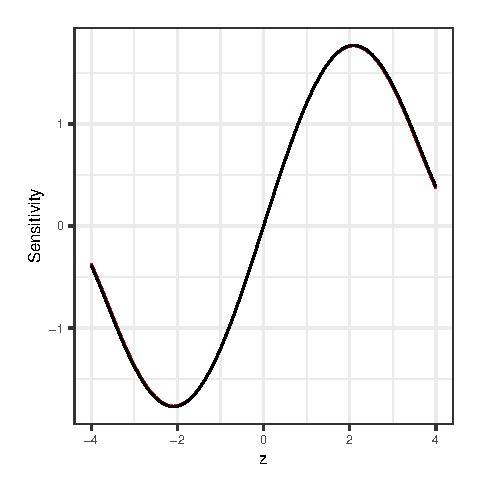
\includegraphics{q1-sens_curves_tukey_large}
    \subcaption{Tukey}
  \end{subfigure}
  \caption{Sensitivity curves (red) based on a symmetric standard normal sample with $n = 1e6$ together with the corresponding influence functions (black)}
  \label{fig:q1-sens-curves-1e2}
\end{figure}

\section*{Question 2}

In the first part of this section, we will analyse the distribution of the \texttt{Copper\_mcg} variable from the food dataset. A QQ-plot against the theoretical quantiles of the standard normal distribution indicates that it is strongly right-skewed, as is often the case when the data are constrained to be positive. Examination of the farthest points in the tail of the distribution reveals that these are all measurements for liver products, and a cursory glance at online resources on nutrition does indeed indicate that this food type is rich in copper (see \cite{liver}). Consequently, it seems plausible that the copper content in the catalogued food items simply follows a fat-tailed distribution.

\begin{figure}[!htb]
  \centering
  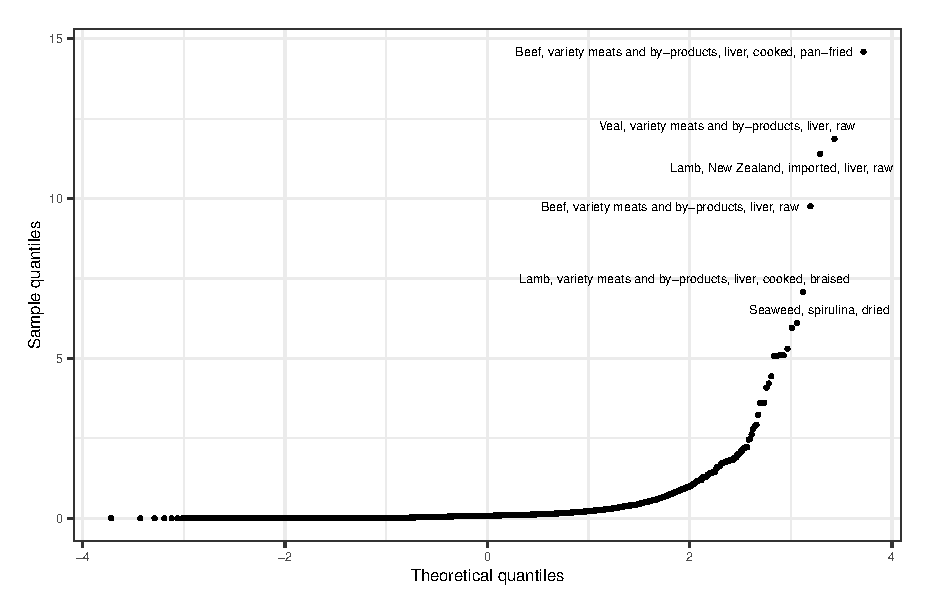
\includegraphics{q2-qq-orig}
  \caption{QQ-plot of \texttt{Copper\_mcg} variable}
  \label{fig:q2-qq-orig}
\end{figure}

Fitting the $\lambda$-parameter for the Box-Cox and Yeo-Johnson transforms using the robust methods implemented in the \texttt{transfo} function from the \texttt{cellWise} package \cite{cellwise}, we obtain estimates of $-0.1061973$ and $0.3051917$, respectively. The resulting QQ-plots are shown in \cref{fig:q2-qq-tf}. Both transforms produce a conspicuous distortion at the lower end of the distribution the right tail, ostensibly in their attempt to capture extreme values in the right tail. Investigation of the horizontal section reveals that it contains points for which the original observations have the same value of \SI{1e-5}{\micro \gram}, which is presumably not an exact measurement but rather a cut-off value. If this is deemed to justify discarding or unifying these observations, then the Yeo-Johnson transform would yield a reasonable approximation to normality, while the Box-Cox transform preserves the right tail. Depending on the interpretation of the extreme points as either outliers or regular observations from a fat-tailed distribution, one result will be preferred over the other.

\begin{figure}[!htb]
  \begin{subfigure}{0.5\linewidth}
    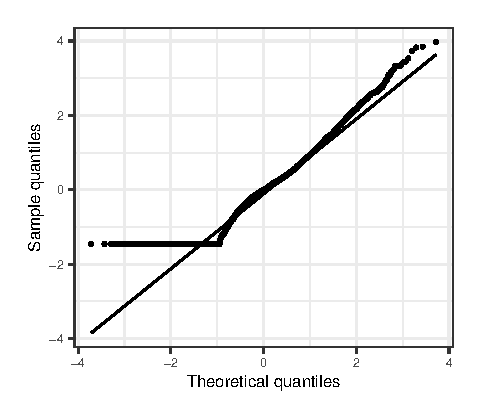
\includegraphics{q2-qq-tf-yj}
    \subcaption{Yeo-Johnson}
  \end{subfigure}
  \begin{subfigure}{0.5\linewidth}
    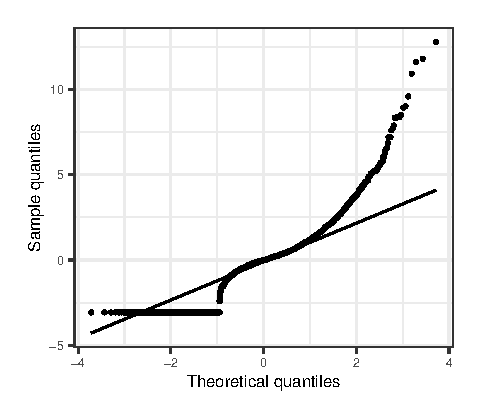
\includegraphics{q2-qq-tf-bc}
    \subcaption{Box-Cox}
  \end{subfigure}
  \caption{QQ-plots of the transformed variable}
  \label{fig:q2-qq-tf}
\end{figure}

Next, we investigate the use of dimensionality reduction techniques for the description of the entire food dataset. Using the ROBPCA procedure implemented in the \texttt{PcaHubert} function of the \texttt{rrcov} package \cite{rrcov} with an initial number $k = 15$ of principal components gives us the screeplot in \cref{fig:q2-scree}, which seems to have an elbow at $k = 6$. Refitting the model with this number yields the loadings matrix shown in \cref{fig:q2-loadings}. Given that the loading vectors constitute an orthonormal basis of the feature space $\mathbb{R}^p$, their Euclidean norm will always equal $1$; hence, it follows that the average value of any loading is $1 / \sqrt{p}$, so that ones which exceed this threshold indicate a salient correlation between the relevant component and the original variable. These are marked in bold in \cref{fig:q2-loadings}.

Without expert knowledge from nutritional science, it seems difficult to derive a clear interpretation from these results. The first two principal components load onto a large number of variables, a number of which are common to both. Nevertheless, there do seem to be two blocks of variables for which there is less overlap, suggesting that these might be somehow related. The third and fourth component are clearly associated with a single one of the original variables (\texttt{VitA\_mcg} and \texttt{Sugar\_g}, respectively), although the latter also exhibits secondary correlations with the surrounding ones. Lastly, the penultimate component exhibits an opposite association of approximately equal strength with two variables, which strongly hints at the presence of an underlying common driver of both, and the final component correlates with many variables, but these notably cover the final block omitted by the PCs $1$ and $2$, which suggest that the three of them might represent global patterns in the data while the remainder account for more concentrated pockets of variation.

With regards to outliers, the plot in \cref{fig:q2-outlier} indicates that all three types are present in this data. For increased interpretability, we augmented the original dataset to include information about the food group of the items using the \texttt{usdanutrients} package \cite{usdanutrients} and highlighted the largest groups for each outlier type in different colours. This reveals that the good leverage points are dominated by the category of Baked Products, with Legumes and Legume Products as a distant second. Breakfast Cereals constitutes the largest group within both orthogonal and bad leverage outliers. Notice that the largest groups of outliers consist of carbohydrate-rich foods, which might aid in interpreting the cause of their deviation.

\newgeometry{bottom=3cm}
\begin{landscape}
  \vfill
  \begin{figure}
    \begin{minipage}{0.5\linewidth}
      \begin{subfigure}{\linewidth}
        \centering
        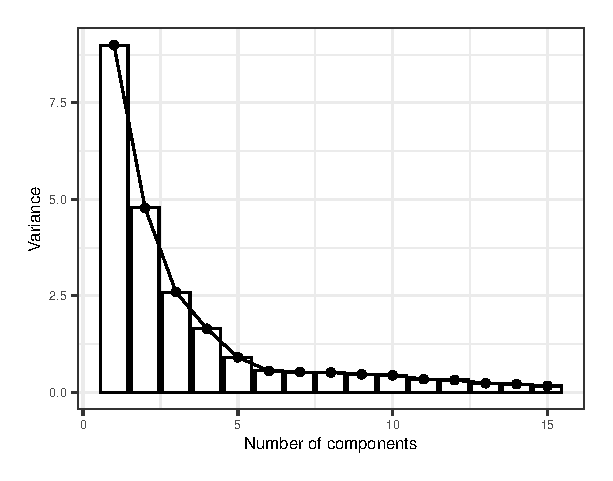
\includegraphics{q2-screeplot}
        \subcaption{Screeplot}
        \label{fig:q2-scree}
      \end{subfigure}
      \begin{subfigure}{\linewidth}
        \centering
        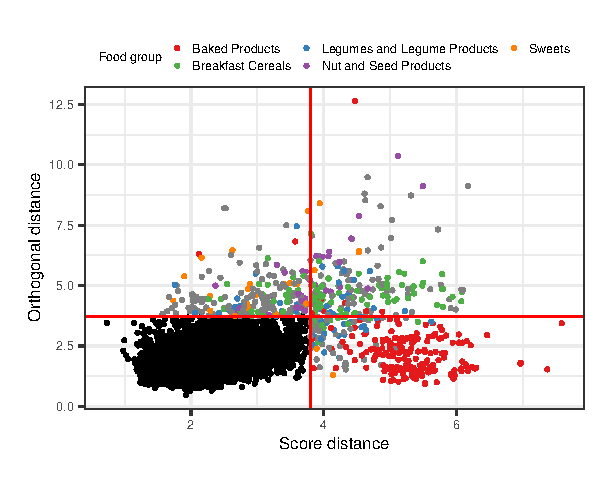
\includegraphics{q2-outlier-plot}
        \subcaption{Outlier plot}
        \label{fig:q2-outlier}
      \end{subfigure}
    \end{minipage}
    \begin{subfigure}{0.5\linewidth}
      \centering
      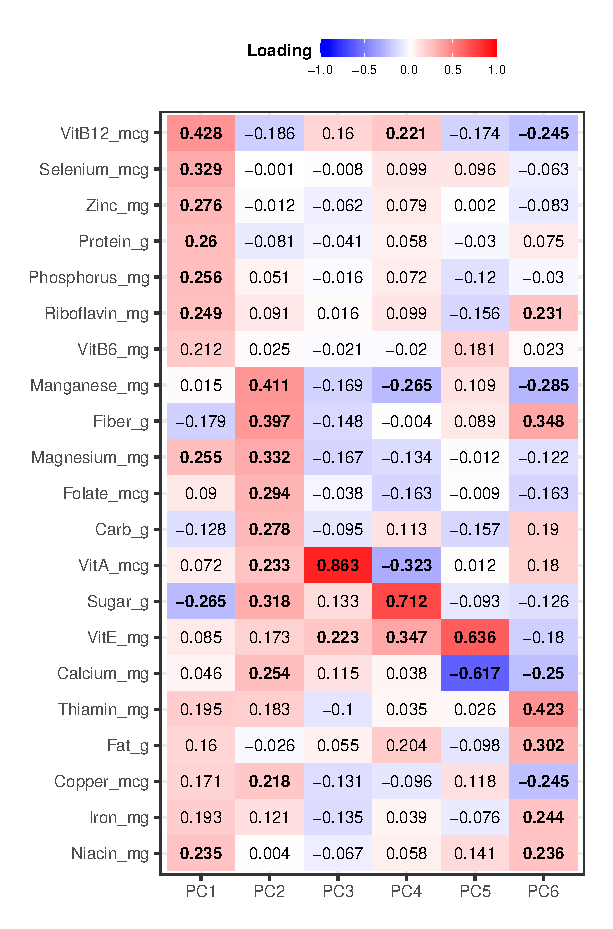
\includegraphics{q2-loadings}
      \subcaption{Loadings}
      \label{fig:q2-loadings}
    \end{subfigure}
    \caption{ROBPCA results}
  \end{figure}
\end{landscape}
\restoregeometry

\section*{Question 3}

Our aim in this section is to construct a normal linear model for predicting the price of a car based on the \texttt{Topgear} dataset. \Cref{tab:q3-summary} shows summary statistics for this response variable. Notice in particular the striking discrepancy between the mean and median, which hints at the presence of outliers in the data.

\begin{table}[!htb]
  \centering
  
\begin{tabular}{@{\hspace{5pt}}lcccccc} 
\toprule 
 
Statistic & \multicolumn{1}{c}{N} & \multicolumn{1}{c}{Mean} & \multicolumn{1}{c}{St. Dev.} & \multicolumn{1}{c}{Min} & \multicolumn{1}{c}{Median} & \multicolumn{1}{c}{Max} \\ 
\midrule \\[-2.1ex] 
Price & 242 & 51,170.54 & 106,879.40 & 7,995 & 26,050 & 1,139,985 \\ 
\bottomrule 
\end{tabular} 

  \caption{Summary statistics for the \texttt{Price} variable}
  \label{tab:q3-summary}
\end{table}

The correlation structure of the continuous variables is visualised in \cref{fig:q3-corplot}. The top row indicates that cars with stronger engines (higher fuel consumption and power, lower acceleration time) generally tend to be more expensive, unsurprisingly. We also observe a high degree of interdependence between the variables of physical measurements (top left square outlined in black), which could lead to issues with multicollinearity.

\begin{figure}[!htb]
  \centering
  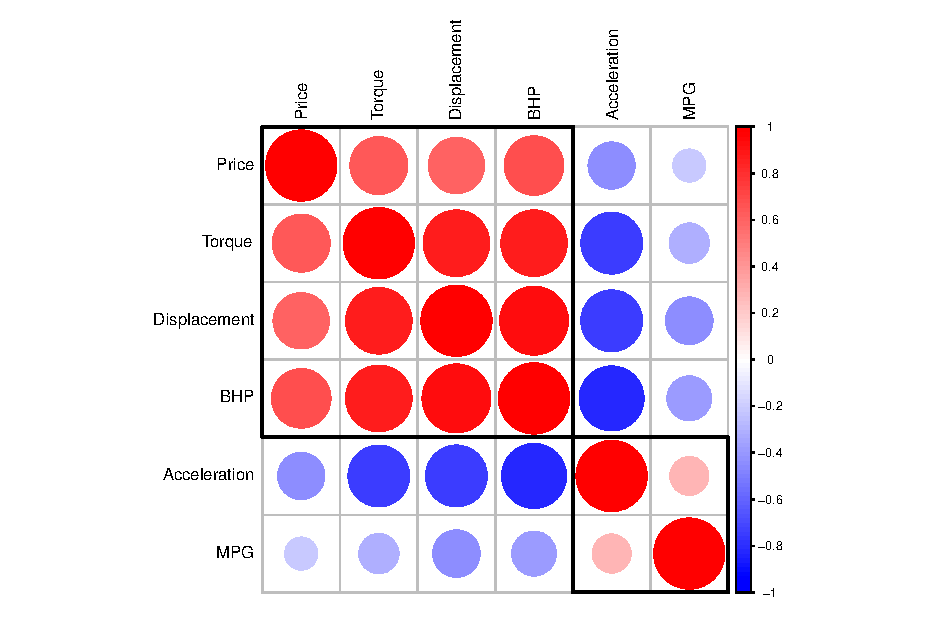
\includegraphics{q3-corplot}
  \caption{Visualisation of the correlation between the continuous variables in the \texttt{Topgear} dataset}
  \label{fig:q3-corplot}
\end{figure}

To assess the appropriateness of the linear model for this dataset, we consider scatterplots of the response against the other continuous variables. The model name being unique to each car, it plays the role of an identifier and is therefore not relevant in this context. The car maker, on the other hand, could very plausibly influence the price. As the number of brands in the dataset is rather high (48 on a total of 242 observations), using this variable as-is would not provide much insight, however. We therefore do a little feature engineering and cluster the makers on the mean price of their cars, dividing them into high, mid and low price categories, which can then be colour coded.

The resulting scatter plots are shown in \cref{fig:q3-scatter-classic}. The observations for the car makers Bugatti and Pagani stand out starkly in all of them, which makes sense, as these are hypercar manufacturers. The data clearly suffers from heteroscedasticity, with higher prices being more dispersed than lower ones. Moreover, while linearity could perhaps seem reasonable within each group separately, it is undeniable that the general slope of the observations changes as we move between groups, contrary to the parallel line pattern we expect from the linear model. Fitting the regression and inspecting the diagnostic plots confirms our suspicions: the graph of the standardised residuals against the fitted values shows a clear downward trend and the distribution of the residuals shows strong deviations from normality in the tails. These findings suggest that the model might benefit from transformation of the response.

\afterpage{
  \newgeometry{left=2cm}
  \begin{landscape}
    \begin{figure}
      \begin{subfigure}{\linewidth}
        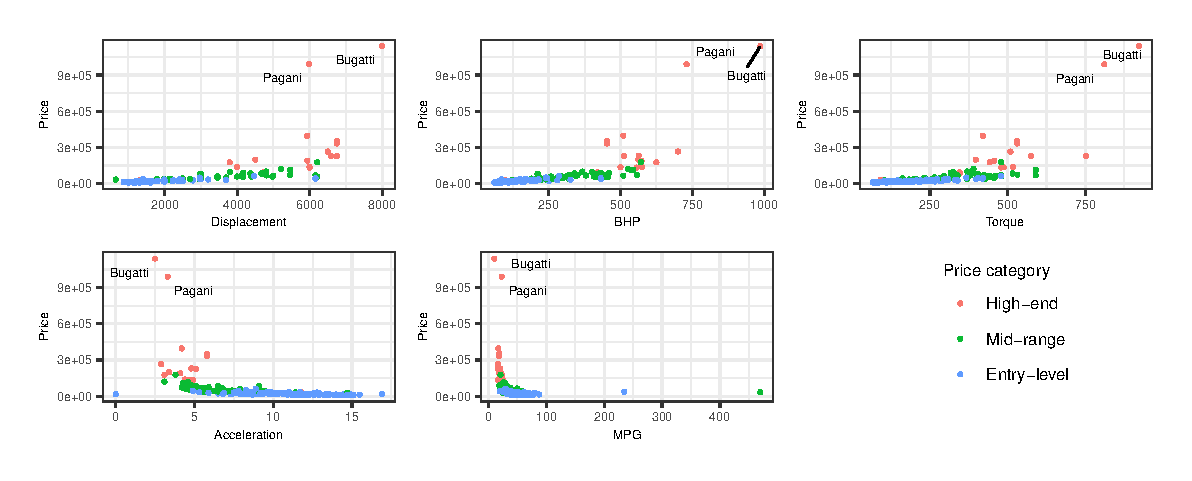
\includegraphics{q3-scatter-classic}
        \subcaption{Original}
        \label{fig:q3-scatter-classic}
      \end{subfigure}
      \begin{subfigure}{\linewidth}
        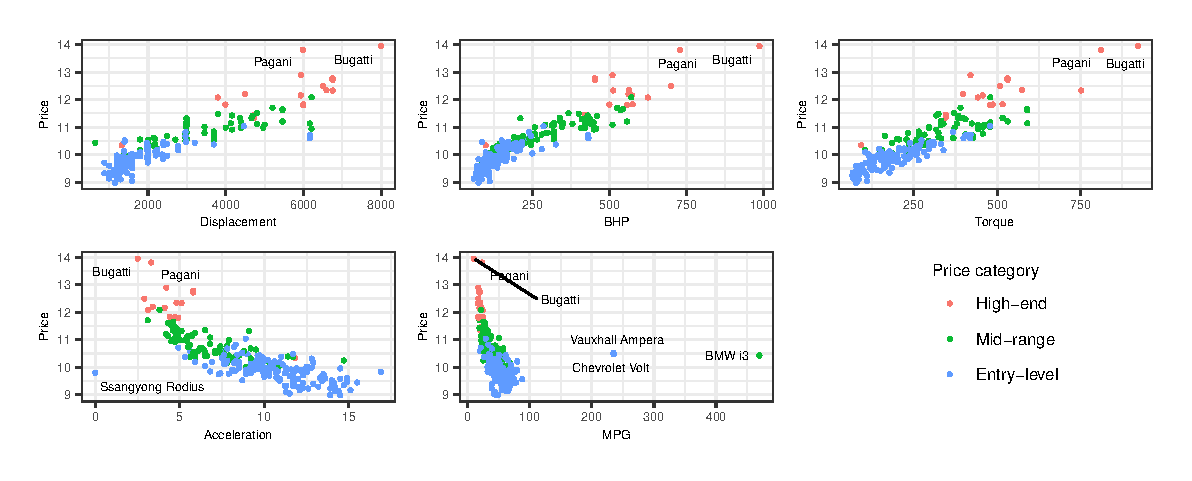
\includegraphics{q3-scatter-tf}
        \subcaption{Transformed}
        \label{fig:q3-scatter-tf}
      \end{subfigure}
      \caption{Scatter plots of the \texttt{Price} variable against the numerical features in the \texttt{Topgear} dataset. The colours indicate different price categories.}
    \end{figure}
  \end{landscape}
  \restoregeometry
}

\begin{figure}[!htb]
  \begin{subfigure}{0.5\linewidth}
    \centering
    \includegraphics{q3-qq-classic}
    \subcaption{Quantile-quantile plot of standardised residuals}
    \label{fig:q3-qq-resp-orig}
  \end{subfigure}
  \begin{subfigure}{0.5\linewidth}
    \centering
    \includegraphics{q3-resids-vs-fitted-classic}
    \subcaption{Studentised residuals vs fitted values}
    \label{fig:q3-resids-vs-fitted-orig}
  \end{subfigure}
  \caption{Diagnostic plots for the linear model}
\end{figure}

Applying a log-transform to the \texttt{Price} variable, we obtain the scatters plots shown in \cref{fig:q3-scatter-tf}. The linear model seems to fit the data much better now: the variance has been stabilised, and the previously observed pattern is gone from \cref{fig:q3-resids-vs-fitted-tf}. Moreover, the hypercar manufacturers which previously stood out like a sore thumb now appear to blend in with the general pattern. However, the number and regularity of outlying residuals in \cref{fig:q3-qq-tf,fig:q3-resids-vs-fitted-tf} can lead one to suspect the presence of fat tails in the price distribution, especially as this is often observed in economic data. Furthermore, we are confronted with some new extreme outliers in the scatterplots for the \texttt{Acceleration} and \texttt{MPG} variables.

The bad leverage of these observations has a severe impact on the linear fit; in particular, it results in a positive coefficient estimate for the \texttt{MPG} variable, which is surprising in view of the expectations expressed earlier on the basis of \cref{fig:q3-corplot}. For the acceleration, closer inspection of the offending observation reveals that it corresponds to a car supposedly able to achieve a speed of \SI{62}{\mph} in \SI{0}{\s}, which is clearly an error. As for the \texttt{MPG} outliers, these correspond to the Chevrolet Volt and Vauxhall Ampera, which are plug-in hybrids, and the BMW i3, which is an electric car. After consulting a domain expert (automotive engineer), it appears that \texttt{MPG} measurements do not incorporate battery consumption for electric-powered vehicules, and are therefore not very meaningful. Based on these considerations, we have chosen to exclude these observations from the remainder of the analysis. Interestingly, neither the classical nor the robust fit were able to identify them as bad leverage points.

\begin{figure}[!htb]
  \begin{subfigure}{0.5\linewidth}
    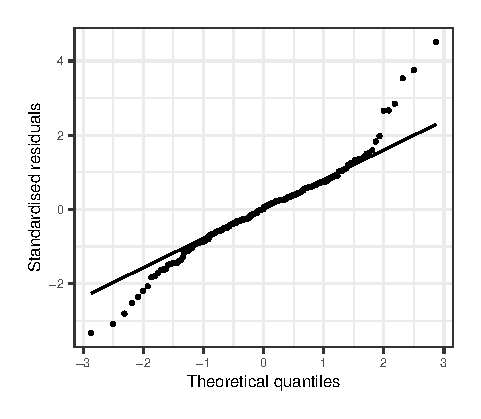
\includegraphics{q3-qq-tf}
    \subcaption{Quantile-quantile plot of standardised residuals}
    \label{fig:q3-qq-tf}
  \end{subfigure}
  \begin{subfigure}{0.5\linewidth}
    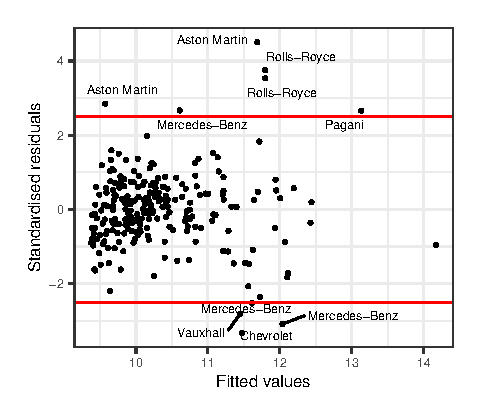
\includegraphics{q3-resids-vs-fitted-tf}
    \subcaption{Studentised residuals vs fitted values}
    \label{fig:q3-resids-vs-fitted-tf}
  \end{subfigure}
  \caption{Diagnostic plots for the normal linear model with log-transformed response.}
\end{figure}

\Cref{tab:q3-reg-res} summarises the regression results for the transformed model under a classical least squares fit, excluding the aforementioned observations. As we can see, they are now consistent with \cref{fig:q3-corplot}, although the fat tails are still present in the residual diagnostics. This makes it difficult to trust parametric significance tests, and have therefore chosen not to include them here. The coefficients are dominated by the intercept term, which not surprising: regardless of its characteristics, a car cannot be sold profitably for few hundred pounds. Moreover, because the response has been log-transformed, these coefficients describe effects \emph{on a multiplicative scale}, i.e.\ they express the \emph{rate} at which the car price increases as a function of the predictors. 

\begin{table}[!htb]
  \centering
  
\begin{tabular}{@{\extracolsep{5pt}} ccccccc} 
\toprule 
 & (Intercept) & Displacement & BHP & Torque & Acceleration & MPG \\ 
\midrule Estimate & $9.29$ & $0.0000$ & $0.003$ & $0.002$ & $$-$0.02$ & $$-$0.001$ \\ 
\bottomrule 
\end{tabular} 

  \caption{Regression results for the linear model with transformed response. The response has been log-transformed and the bad observations excluded.}
  \label{tab:q3-reg-res}
\end{table}

\newgeometry{top=2cm,bottom=2cm}
\begin{figure}[!htb]
  \begin{subfigure}{0.5\linewidth}
    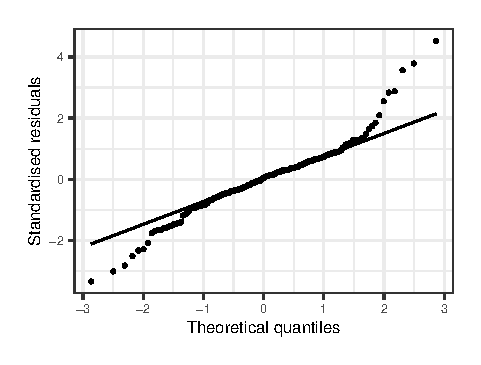
\includegraphics{q3-qq-corrected}
    \subcaption{Quantile-quantile plot of standardised residuals}
    \label{fig:q3-qq-corrected}
  \end{subfigure}
  \begin{subfigure}{0.5\linewidth}
    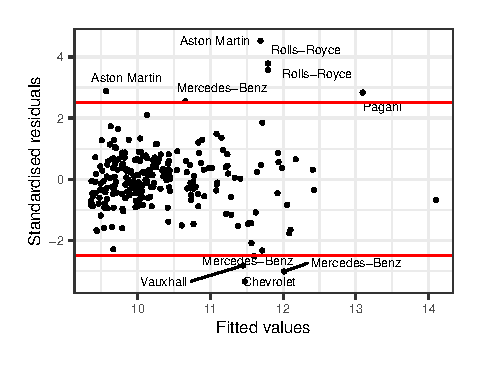
\includegraphics{q3-resids-vs-fitted-corrected}
    \subcaption{Studentised residuals vs fitted values}
    \label{fig:q3-resids-vs-fitted-corrected}
  \end{subfigure}
  \caption{Diagnostic plots for the linear model. The response has been log-transformed and the bad observations excluded.}
\end{figure}

Finally, we repeat the previous analysis using the robust LTS fit in place of the classical one. The model diagnostics are broadly the same, but the robust fit flags many more observations as good leverage outliers than the least squares one does. Moreover, the deviation in the tails is slightly more pronounced, as can be seen more clearly by comparing the outlier maps in \cref{fig:q3-outlier-maps}. The persistence of these phenomena is worrying and leads us to suspect one of two things: either the Gaussian distribution must be replaced by a more appropriate one, or there is some pattern in the data which our model fails to capture. Looking back at the scatterplots in \cref{fig:q3-scatter-tf}, we conjecture that there might be groupwise effect between the different price categories which is unaccounted.

\begin{table}[!htb]
  \centering
  
\begin{tabular}{@{\extracolsep{5pt}} ccccccc} 
\toprule 
 & Intercept & Displacement & BHP & Torque & Acceleration & MPG \\ 
\midrule Estimate & $9.34$ & $0.0000$ & $0.003$ & $0.002$ & $$-$0.02$ & $$-$0.0000$ \\ 
\bottomrule 
\end{tabular} 

  \caption{Regression results for the linear model with robust fit. The response has been log-transformed and the bad observations excluded.}
  \label{tab:q3-reg-res-rob}
\end{table}

\begin{figure}[!htb]
  \begin{subfigure}{0.5\linewidth}
    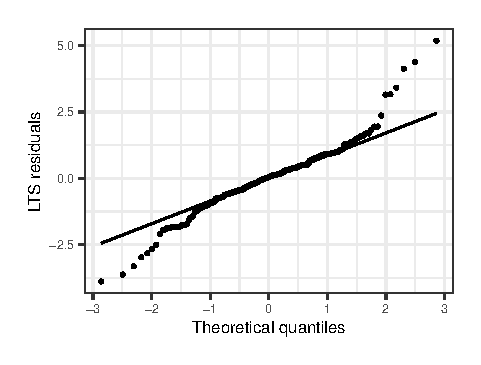
\includegraphics{q3-qq-rob}
    \subcaption{Quantile-quantile plot of standardised residuals}
    \label{fig:q3-qq-resp-rob}
  \end{subfigure}
  \begin{subfigure}{0.5\linewidth}
    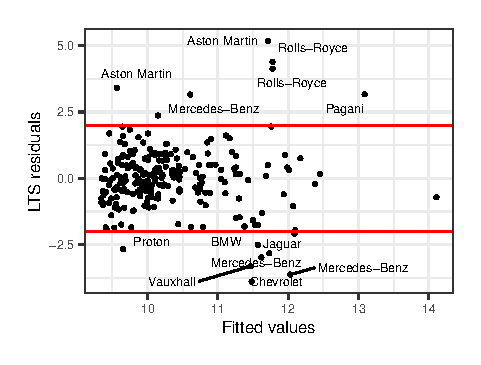
\includegraphics{q3-resids-vs-fitted-rob}
    \subcaption{Studentised residuals vs fitted values}
    \label{fig:q3-resids-vs-fitted-rob}
  \end{subfigure}
  \caption{Diagnostic plots for linear model with robust fit. The response has been log-transformed and the bad observations excluded.}
\end{figure}
\restoregeometry

\begin{landscape}
  \begin{figure}
    \begin{subfigure}{0.5\linewidth}
      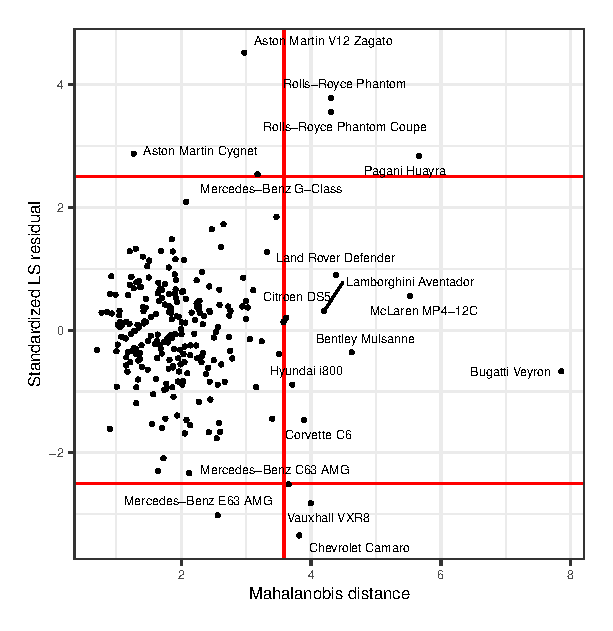
\includegraphics{q3-outlier-classic}
      \caption{Classical LS fit}
      \label{fig:q3-outlier-classic}
    \end{subfigure}
    \begin{subfigure}{0.5\linewidth}
      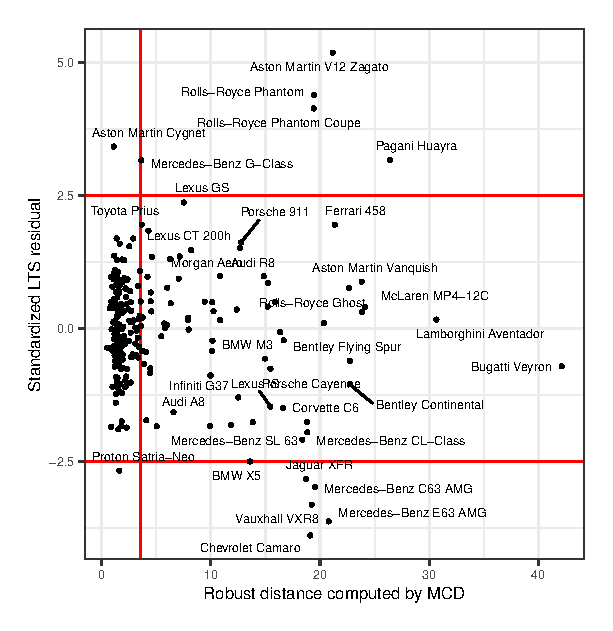
\includegraphics{q3-outlier-rob}
      \caption{Robust LTS fit}
    \end{subfigure}
    \caption{Outlier maps}
    \label{fig:q3-outlier-maps}
  \end{figure}
\end{landscape}

Refitting the model a final time while incorporating the price category variable, we obtain the diagnostic plots displayed in \cref{fig:q3-qq-resp-price-cat,fig:q3-resids-vs-fitted-price-cat}, which show notable improvement. While the residuals still exhibit heavier tails than would warranted under normality, the deviation does not appear to be so significant as to invalidate inferences made on this basis; in fact, both the Shapiro-Wilk and Anderson-Darling tests fail to reject normality of the residuals at a significance level of $0.05$, though the former only narrowly.

\begin{table}[!htb]
  \centering
  \makebox[\textwidth][c]{% latex table generated in R 4.1.3 by xtable 1.8-4 package
% Mon May 29 12:31:12 2023
\begin{tabular}{rrrrrrrrr}
  \toprule
 & (Intercept) & Displacement & BHP & Torque & Acceleration & MPG & CatMid-range & CatEntry-level \\ 
  \midrule
Estimate &  10 & 3e-05 & 0.0014 & 0.0022 & -0.02 & -0.0015 & -0.61 & -0.86 \\ 
  p-value & 2.3e-132 & 0.35 & 0.00033 & 3.4e-18 & 0.039 & 0.34 & 5.4e-14 & 1.4e-19 \\ 
   \bottomrule
\end{tabular}
}
  \caption{Regression results for the linear model with classical fit. The response has been log-transformed and the bad observations excluded.}
  \label{tab:q3-reg-res-price-cat}
\end{table}

\begin{figure}[!htb]
  \begin{subfigure}{0.5\linewidth}
    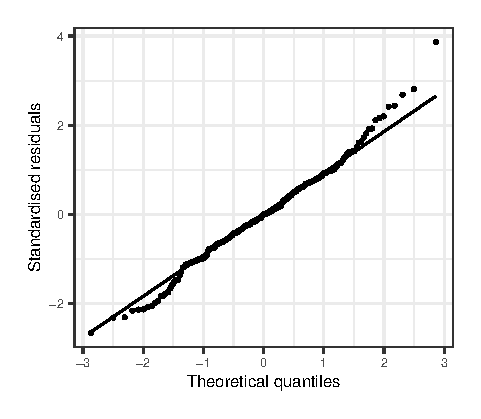
\includegraphics{q3-qq-price-cat}
    \subcaption{Quantile-quantile plot of standardised residuals}
    \label{fig:q3-qq-resp-price-cat}
  \end{subfigure}
  \begin{subfigure}{0.5\linewidth}
    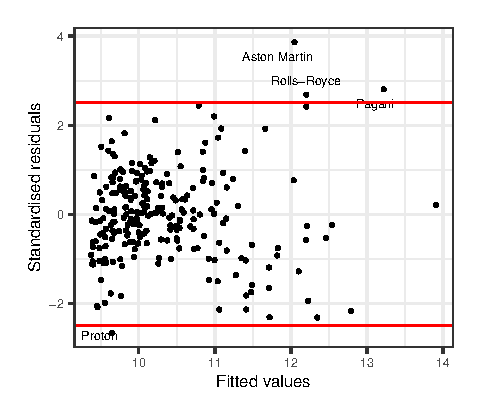
\includegraphics{q3-resids-vs-fitted-price-cat}
    \subcaption{Studentised residuals vs fitted values}
    \label{fig:q3-resids-vs-fitted-price-cat}
  \end{subfigure}
  \caption{Diagnostic plots for linear model with classical fit. The response has been log-transformed and the bad observations excluded.}
\end{figure}

Once again, the sign of the coefficients agrees with the correlations for the continuous variables, and makes logical sense for the newly introduced categorical one. Moreover, significant effects are only present for 2 out of 3 variables from the first feature group in \cref{fig:q3-corplot} and 1 out of 2 from the second, which is consistent with the dependency structure observed there.

\section*{Question 4}

The \texttt{warpbreaks} dataset contains observations of the number of breaks in yarn during weaving for different types of wool (A and B) and levels of tension (low, medium and high). In this section, we will be interested in predicting the number of breaks as a function of the wool type and tension level. A boxplot indicates the existence of an inverse relation between the response and the latter of these variables.

\begin{figure}[!htb]
  \centering
  \label{fig:q4-boxplot}
  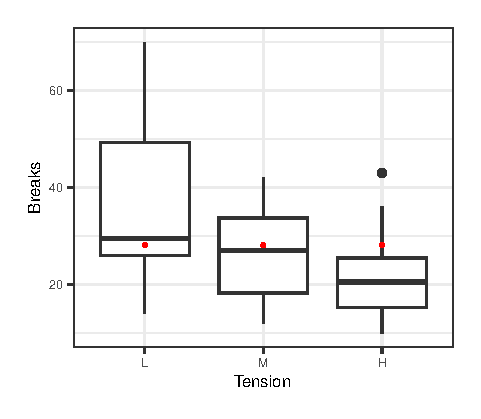
\includegraphics{q4-boxplot}
  \caption{Boxplot of response at the different levels of tension. The mean is indicated in red.}
\end{figure}

As the response consists of counts, the data lends itself naturally to a Poisson GLM. The independent variables are categorical in nature and must therefore be converted using some kind of encoding scheme before the model can be fitted. The default one used in \texttt{R} is dummy encoding, where a binary vector is used to indicate which levels are present for a particular observation. Note that the indicator vector for a categorical variable with $k$ levels will have only $k - 1$ entries, otherwise the model would not be identifiable. The resulting design matrix will be an array with values in $\{0, 1 \}$, of which the first few rows are shown in \cref{tab:q4-design-mat}.

\begin{table}[!htb]
  \centering
  
\begin{tabular}{@{\extracolsep{5pt}} ccccc} 
\toprule 
 & (Intercept) & woolB & tensionM & tensionH \\ 
\midrule 1 & $1$ & $0$ & $0$ & $0$ \\ 
2 & $1$ & $0$ & $0$ & $0$ \\ 
3 & $1$ & $0$ & $0$ & $0$ \\ 
4 & $1$ & $0$ & $0$ & $0$ \\ 
5 & $1$ & $0$ & $0$ & $0$ \\ 
6 & $1$ & $0$ & $0$ & $0$ \\ 
\bottomrule 
\end{tabular} 

  \caption{First few rows of the design matrix}
  \label{tab:q4-design-mat}
\end{table}

\Cref{tab:q4-glm-res} shows the results of fitting the Poisson regression $\texttt{breaks} \sim \texttt{wool} + \texttt{tension}$ to the \texttt{warpbreaks} dataset. As expected, the coefficient estimate becomes more negative for higher levels of tension. It is important to bear in mind, however, that this model uses a log link, so that these numbers express effects on a multiplicative scale. All coefficient estimates are found to be significant, but the p-values can only be trusted if the model assumptions are fulfilled.

\begin{table}[!htb]
  \centering
  
\begin{tabular}{@{\hspace{5pt}}l@{\hspace{5pt}}c} 
\toprule 
 & \multicolumn{1}{c}{\textit{Dependent variable:}} \\ 
\cmidrule(rr){2-2} 
 & breaks \\ 
\midrule  
\\[-2.1ex] woolB & $-$0.206$^{***}$ (0.052) \\ 
  tensionM & $-$0.321$^{***}$ (0.060) \\ 
  tensionH & $-$0.518$^{***}$ (0.064) \\ 
  Constant & 3.692$^{***}$ (0.045) \\ 
 \midrule  
Observations & 54 \\ 
Log Likelihood & $-$242.528 \\ 
Akaike Inf. Crit. & 493.056 \\ 
\bottomrule 
\textit{Note:}  & \multicolumn{1}{r}{$^{*}$p$<$0.1; $^{**}$p$<$0.05; $^{***}$p$<$0.01} \\ 
\end{tabular} 

  \caption{Results for the Poisson GLM}
  \label{tab:q4-glm-res}
\end{table}

To check for the presence of overdispersion in the data, we consider the plot of response against the fitted value given in \cref{fig:q4-resp-fit-pois}. The bars show 95\% confidence intervals under the Poisson GLM. A significant number of observations fall outside of this range, suggesting that the data exhibits more variability than is appropriate for the model. A formal test using the \texttt{dispersiontest} function from the \texttt{AER} package \cite{aer} (which is based on \cite{cameron}) confirms our suspicion, rejecting the null hypothesis of unit dispersion with $p = $ \SI{2.33e-06}. The significance tests for the coefficients shown earlier are therefore unreliable.

To account for this, we adjust the GLM to use the quasi-Poisson family, which allows the dispersion parameter $\phi$ to be greater $1$. The resulting diagnostic plot, shown in \cref{fig:q4-resp-fit-pois}, looks much better. Note that the bars represent a range of $3$ estimated standard deviations around the fitted mean.

\begin{figure}[!htb]
  \centering
  \begin{subfigure}{0.45\linewidth}
    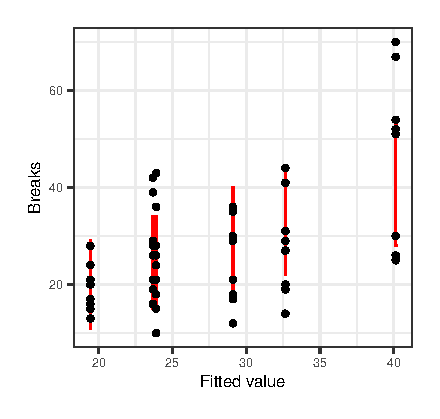
\includegraphics{q4-resp-fit-pois}
    \centering
    \subcaption{Poisson}
    \label{fig:q4-resp-fit-pois}
  \end{subfigure}
  \begin{subfigure}{0.45\linewidth}
    \centering
    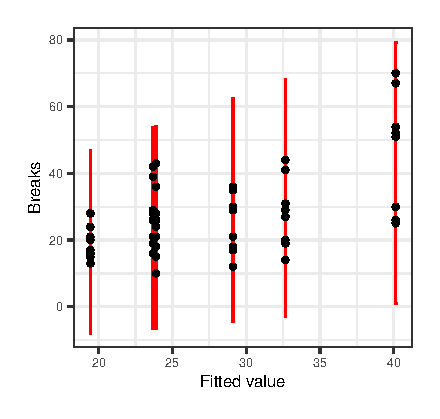
\includegraphics{q4-resp-fit-quasi}
    \subcaption{Quasi-Poisson}
    \label{fig:q4-resp-fit-quasi}
  \end{subfigure}
  \caption{Response against fitted value}
\end{figure}

Finally, we repeat the same analysis using a robust estimator. As we were unable to find an implementation supporting the quasi-Poisson family, we will use the ordinary variant and limit ourselves to comparison of coefficients. As we can see in \cref{tab:q4-rob-res}, these are broadly similar, increasing our confidence in the previous model.

\begin{table}[!htb]
  \centering
  
\begin{tabular}{@{\extracolsep{5pt}} ccccc} 
\toprule 
 & (Intercept) & woolB & tensionM & tensionH \\ 
\midrule Estimate & $3.56$ & $$-$0.15$ & $$-$0.23$ & $$-$0.45$ \\ 
\bottomrule 
\end{tabular} 

  \caption{Results for the Poisson GLM with robust fit}
  \label{tab:q4-rob-res}
\end{table}

\clearpage

\printbibliography%

\end{document}